As early as 2001, researchers have proposed the use of a novel, hybrid engine
design for use in supersonic and hypersonic flight \cite{Macheret2001}. In some
ways similar to an earlier program \cite{Gurijanov1996}, it suggested that
magnetohydrodynamic (\acs{mhd}) accelerators were an enabling technology for
hypersonic transport. Briefly, a \acs{mhd} accelerator could be used to
simultaneously produce energy and slow the inlet airflow. This would allow the
use of a conventional turbojet engine at speeds well above its normal
operational range.

However, \acs{mhd} accelerators require an ionized fluid flow. Even at the high
altitudes associated with hypersonic flight, this is not easy to achieve.
Originally, Macheret suggested the use of electron beams, carefully tuned to
coincide with the peak in the ionization cross section in air. However, the use
of electron beams in the ionization of high pressure gases is accompanied by a
large number of technical issues, similar to those of some excimer lasers.
Therefore, in 2002, Macheret et al.\ proposed the use of a \acs{rpnd} to produce
an ``electron beam'' in situ \cite{Macheret2002} akin to the beams observed in
certain \acs{fiw} studies.

The use of a \acs{rpnd} is accompanied by a reduced ionization efficiency in
comparison to an electron beam. However, it reduces the some of the
implementation challenges and Macheret argued that it offered a more efficient
and stable option than breakdown with DC electric fields. Though the densities
of \acs{fiw}s in several air-related chemistries have been measured on several
occassions \cite{Anikin1998, Aleksandrov2007, Aleksandrov2008,
Starikovskaia2006}, similar studies do not appear to exist for \acs{rpnd}s in
air. Therefore, there is a need for electron density measurements to confirm
that \acs{rpnd}s are adequate for the \acs{mhd} accelerator requirements and to
quantify their ionization efficiency.

In addition, previous studies of \acs{fiw}s in air have observed fast gas
heating of molecular systems \cite{Popov2011}. Up to 40\% of the input energy
can be converted into translational energy through dissociation of oxygen and
quenching or electronically excited nitrogen states. As the \acs{rpnd} physics
are very similar to that of the \acs{fiw}, there is the possibility that it may
also cause fast gas heating. In combustion, this can play an important role in
the chemistry, flame holding, and ignition delay. More generally, gas heating
can impact material processing and ionization efficiency. As such, it is
important to develop reliable temperature diagnostics for \acs{rpnd}s in
molecular gases.

This appendix records the development of two diagnostics for an air \acs{rpnd}
at \acs{nasa} Glenn Research Center (\acs{grc}). Measurement of the electron
density was accomplished using millimeter-wave interferometry. Plasma
interferometry measures changes in the phase and amplitude of an electromagnetic
wave which has passed through the plasma \cite{Lieberman2005}. The phase shift
is proportional to the density of electrons while the change in amplitude is
related to the electron-neutral collision frequency. As with other wave-based
techniques, the density resulting from this approach is line integrated. The
translational temperature of the system was measured via

Translational temperatures were measured by analysis of the rotational spectra
associate with the second positive system of nitrogen. Rotational spectra result
from changes in the rotational quanta of a molecule. As the energy spacing of
the rotational levels is generally quite small (often on the order of $10^{-4}$
eV), inter-molecular collisions can easily redistribute them
\cite{Herzberg1950}. Provided enough collisions, the distribution of rotational
states should reflect the distribution of translational energy for the
molecules.

\section{Discharge Apparatus}\label{sec:apparatus2}

Experiments were conducted in a cylindrical vacuum chamber, reproduced in
figure~\ref{fig:nasachamber},
\begin{figure}
  \centering
  \setlength\fboxsep{0pt}
  \setlength\fboxrule{1.0pt}
  \fbox{\includegraphics{./chapters/nasa/figures/VF-69.jpg}}
  \caption{Vacuum chamber used in \acs{rpnd} experiments at the \acs{nasa}
    \acs{grc} along with an intensified \acs{ccd} used for fast imaging.}
  \label{fig:nasachamber}
\end{figure}
with a volume of approximately 30 L. The chamber was evacuated by a Varian
TriScroll 300, scroll pump and the pressure was monitored by a capacitance
manometer. Before each experiment the chamber pressure was reduced to below 100
mTorr, after which the chamber was sealed from the pump by a bellows valve. The
chamber was then back-filled with ambient air until the pressure reached 20.0
Torr.

The discharge was sustained between two parallel cylindrical electrodes, 2.5 cm
in diameter and 0.625 cm in length. In the interferometry experiment, the
electrodes were mounted in a silicone-based dielectric epoxy, cast such that it
was flush with the faces of the electrodes. Optical emission experiments
eliminated the dielectric epoxy in favor of a machinable ceramic and slightly
different geometry, seen in figure~\ref{fig:electrodes}.
\begin{figure}
  \centering
  \includegraphics{./chapters/nasa/figures/electrodes.pdf}
  \caption{The electrodes used in the \acs{rpnd} at \acs{nasa} \acs{grc}. The
    electrodes are made of copper with a ceramic sheath made of Mykroy.}
  \label{fig:electrodes}
\end{figure}
This choice was made as a result of damage observed to the epoxy molds. Plasma
breakdown appeared to be occurring at the interface of the mold and the
electrodes. The use of the Mykroy fitting allowed longer duration operation
necessary for the optical emissions measurements.

The power supply was built by FID (model FPG 60-100-MC4-S5) and supplied voltage
pulses of up to 60 kV at repetition rates from 6-100 kHz with pulsewidths of 5
ns. Unless otherwise stated, all measurements were made with the power supply
operating at 20 kHz using a Wavetek FG3C as the master clock.

Maintenance of the electrodes and other components of the discharge apparatus
required that the chamber volume regularly be brought up to atmospheric
pressure. When the discharge was initiated after the chamber was returned to the
20.0 Torr operating pressure, a pressure transient was observed. This transient
caused the chamber pressure to rise by about 2.0 Torr after several minutes of
operation, after which the pressure would remain relatively stable. This was
believed to be caused by the outgassing of the discharge apparatus surfaces.
Throughout operation, the pressure would continue to increase at a greatly
reduced rate, on the order of several tenths of a Torr per minute.

\section{Millimeter-Wave Interferometry}

Traditionally, plasma interferometry has been conducted with microwaves, as the
electron densities in processing plasmas cause readily observable phase shifts
at these wavelengths. However, results from similar \acs{rpnd}s
\cite{Starikovskaia2001} suggested that the electron densities could approach
$10^{13}$ cm$^{-3}$. Such densities exceed the cutoff wavelength of microwave
interferometers \cite{Lieberman2005}. As a result, it was necessary to use
millimeter-wave (\acs{mmw}) interferometry which uses much higher frequencies in
order to avoid this issue.

\subsection{Theory}

The theory underlying interferometry can be found in many plasma diagnostic
textbooks, however the majority of the treatments only concern plasmas in which
there are no neutral particles. In contrast, the work of Akhtar et al.
\cite{Akhtar2003} introduces a frictional force to the derivation which accounts
for the effects of neutral particles. Following this approach, the theory below
provides the necessary set of equations in order to determine the electron
density and collision frequency provided measurements of the \acs{mmw} phase
shift and change in amplitude.

The derivation begins with the motion of electron in an oscillating
electromagnetic field. The position of a charged particle in such a field can be
found from the non-relativistic Lorentz equation,
  \begin{equation}
    \bm{F} = q\left( \bm{E} + \bm{v} \times \bm{B} \right),
    \label{eqn:lorentz}
  \end{equation}
where $\bm{F}$ is the force on the particle, $q$ is its charge, $\bm{E}$ is the
electric field, $\bm{v}$ is the particle's velocity, and $\bm{B}$ is the
magnetic field. In the case of a weak electromagnetic field (such as in
interferometry) the magnetic field component can be assumed to be zero. Without
loss of generality, the equation may be reduced to a single dimension.
Afterward, the drag force which accounts for the neutral particle collisions can
be introduced. The acceleration of the electron can then be written as
  \begin{equation}
    \ddot{r} = -\frac{e E}{m} - \nu_\mathrm{eff} m_e \dot{r},
  \end{equation}
where $r$ is the position of the electron, $e$ is the elementary charge,
$\nu_\mathrm{eff}$ is the effective rate of momentum transfer, and $m_e$ is the
mass of the electron.

The electric field of the incident \acs{mmw} can be expressed as $E_0 e^{i\omega
t}$ where $E_0$ represents the peak field strength and $\omega$ is the angular
frequency. The form of $E$ suggests a sinusoidal solution such that $r \propto
e^{i\omega t}$. Solving the differential equation for $\dot{r}$ yields
  \begin{equation}
    \dot{r} = -\frac{eE}{m_e}\frac{\nu_\mathrm{eff} + i\omega}
                                  {\nu_\mathrm{eff}^2 + \omega^2}.
  \end{equation}
This is the drift velocity of the electron. It can be used to solve for the
complex plasma conductivity and, subsequently, the dielectric constant. This
allows one to write the complex propagation coefficient for the \acs{mmw},
  \begin{equation}
    \gamma = \alpha + i\beta,
  \end{equation}
where the real component, $\alpha$, results in a decay of the wave amplitude.
$\beta$ on the other hand, induces a phase shift in the wave. The full solution
for the separate propagation components is given by Akhtar \cite{Akhtar2003} as,
\newcommand{\ts}{\frac{\omega_p^2}{\omega^2 + \nu_\mathrm{eff}^2}}
\begin{align}
  \beta & = \frac{\omega}{c} \left\{ \frac{1}{2} \left(1 - \ts \right)
          + \frac{1}{2} \left[ \left( 1 - \ts \right)^2
          + \left( \ts \frac{\nu_\mathrm{eff}}{\omega} \right)^2
              \right]^{1/2} \right\}^{1/2}, \\
    \alpha & = \frac{\omega}{c} \left\{ -\frac{1}{2} \left(1 - \ts \right)
          + \frac{1}{2} \left[ \left( 1 - \ts \right)^2
          + \left( \ts \frac{\nu_\mathrm{eff}}{\omega} \right)^2
              \right]^{1/2} \right\}^{1/2}.
\end{align}
From these components, explicit solutions can be derived for the electron
density and effective collision frequency,
\begin{align}
  \nu_\mathrm{eff} & = 2 \frac{c^2}{\omega}\frac{\alpha\beta}{\xi}, \\
  n_e & = \frac{m_e\epsilon_0}{e^2}\xi
         \left(\omega^2+\nu_\mathrm{eff}^2\right), 
\end{align}
where $\xi = 1 - (\beta^2-\alpha^2)c^2/\omega^2$. The values for $\alpha$ and
$\beta$ come from the experimental measures of the phase shift and change in
amplitude,
    \begin{align}
        \Delta \phi &= \int_0^d \left( \beta_0 - \beta\right)dr, \qquad
        \textrm{and} \\
        \Delta A &= \int_0^d \left( \alpha_0 - \alpha \right)dr,
    \end{align}
where $\Delta \phi$ is the phase change, $\Delta A$ is the amplitude change, $d$
is the pathlength through the plasma, and $\alpha_0$ and $\beta_0$ are free
space propagation values. As any measurements are integrated over the pathlength
of the system, it is necessary to make some assumption about the variation of
the density with respect to the path of the wave. In this case, the density will
be assumed to be constant along the path of the wave.

\subsection{Experiment}

The \acs{mmw} interferometry was conducted using an HP 8510C network analyzer
operating at 75 GHz. The network analyzer was controlled by a LabView script and
had a maximum sample rate of 5 Hz. Each sample required approximately 100 $\mu$s
to complete.

The \acs{mmw} signal was transmitted between two test sets which produced a
variable frequency signal covering all of the V band (50-75 GHz). The output of
each test set was connected to a high gain horn. The horns were aligned
perpendicular to the axis of the discharge and transmitted through quartz
windows on either side of the vacuum chamber. The horns were aligned by a
maximization of the transmission through the chamber. During data analysis, the
pathlength of the signal through the plasma was assumed to be 2.5 cm, however
diffusion results in the transport of electrons outside of the discharge region,
making this value an underestimate.

During operation, the actual pressures within the vacuum chamber varied from
19.9 to 22.6 Torr. The power supply was operated in a bipolar mode with one
electrode pulsed to $+9$ kV and the other pulsed to $-9$ kV. Previous interest
in the use of a DC sustainer discharge \cite{Schneider2009a} prompted an
investigation of the effects of the sustainer on the time-averaged electron
density. The sustainer consisted of a pair of floating electrodes, perpendicular
to the \acs{rpnd}. The sustainer electrodes were held at a potential difference
that was slightly less than the DC breakdown voltage. The intended effect of the
sustainer was to increase the time-averaged plasma density through additional
ionization.

\subsection{Results}

The original intent was to obtain a measurement of the electron density as it
evolved during and after the pulse. However, the acquisition rate of 5 Hz
prevented acquisition of the electron density evolution for a single pulse.
Instead, it necessitated measurements spanning several minutes and many
thousands of pulses. This made it necessary to determine the repeatability of
the plasma produced by these pulses.

This is generally not an issue in systems which feature gas flows, such as those
studied by Adamovich et al. \cite{Adamovich2009}. However, in this case, the
vacuum chamber was sealed. This mode of operation can cause a slow accumulation
of chemical species, increases in gas temperature, deposits on electrode
surfaces, and more. Each of these has the ability to slowly alter the nature of
the discharge and can complicate analysis of data acquired after different
pulses.

Measurements were made of the electron density for a period of 30 minutes at a
rate of 5 Hz. A SRS DG535 was used to trigger the network analyzer at the same
delay after each pulse. Acquisition for longer periods were prevented as a
result of significant electromagnetic interference \acs{emi}. The master clock
was particularly susceptible to this electrical noise. This would occasionally
shut off the triggering signal or alter its frequency. Several attempts were
made to limit the interference to the signal generator through shielding of the
transmission cables and of the signal generator, however these attempts resulted
in minimal benefit.

Figure~\ref{fig:densev}
\begin{figure}
  \centering
  \includegraphics{./chapters/nasa/figures/densev.pdf}
  \caption{The evolution of the density (---) and the collision frequency
    (\raisebox{2.5pt}{${\scriptscriptstyle \centerdot \centerdot \centerdot}$}) in
    a \acs{rpnd} over a period of 30 minutes. These quantities reach their
    respective maximum and minimum after approximately five minutes, however these
    are not equilibrium values. The \acs{rpnd} continues to change over long
    durations.}
  \label{fig:densev}
\end{figure}
shows the calculation of the electron densities and collision frequencies from
the measured phase and amplitude changes. The data shown does not include the
operation of the DC sustainer. The data appear to confirm the concern that the
sealed vacuum chamber causes long-term variations in the plasma. The electron
density changes by nearly 50\% during the first five minutes of operation and is
followed by a slow decline over the next 25 minutes. Overall, the electron
density ranged from 2.25-3.25 $\times10^{11}$ cm$^{-3}$. This is somewhat less
than the anticipated density. As previously noted, other studies in \acs{fiw}
discharges \cite{Aleksandrov2007, Pancheshnyi1999, Macheret2006} measured
densities well in excess of 10$^{12}$ cm$^{-3}$. Separate experiments
demonstrated similar electron densities. In each case, changes in the electron
density occurred relatively slowly after the first ten minutes. The complex
chemistry of air plasmas makes it difficult attribute the changes in electron
density to a specific process. More likely is a number of subtle changes
throughout the convoluted reaction chains that pertain to air plasmas.

The collision frequency also exhibits changes on a time scale similar to that of
the electron density. It begins quite high before quickly declining to a
minimum, followed by a slow return to its original value. While the pressure
changes by several percent over the course of operation, this is not large
enough to explain the variation in collision frequency. Additionally, the trend
in electron density is opposite of what would be necessary to explain the
observed changes. The average electron temperature between pulses is almost
certainly changing over time. The resulting changes in the interaction cross
sections may be sufficient to explain the change in the collision frequency.
The changes might also be explained by slow evolutions in the relative gas
composition.

\subsection{DC Sustainer}

Six separate experiments were run with the DC sustainer discharge activated. In
each case, the potential difference between the sustainer electrodes was fixed
at 750 V. These experiments were to be compared to the result with the sustainer
turned off. However, \acs{emi} caused the triggering signal generator to fail
before any case could be run to completion. This makes it impossible to come to
any firm conclusion on the impact of the sustainer. For the data that are
available, the DC sustainer \emph{reduced} the overall density of the
\acs{rpnd}.

This reduction in electron density was not originally expected and should be
more thoroughly investigated with a more robust apparatus. It is believe that
the sustainer's predominant effect was an increased energy transfer to the
excited rotational and vibrational states of the molecules.

It is believed that the sustainer may have caused increased energy transfer to
the excited states of atoms and molecules, but was ineffective at increasing the
electron density. Indeed, the sustainer voltage was insufficient to produce a
glow discharge independent of the high voltage pulses. As such, one may conclude
that it will tend to extract more electrons than it produces. This being the
case, a DC sustainer may be useful in situations requiring fast gas heating, but
at the cost of a reduced ionization efficiency. followed by a slow decline over
the next 25 minutes. Simultaneously, the effective collisions frequency of the
electrons ranges from 10-18 GHz. Overall, the electron density ranged from
2.25-3.25 $\times10^{11}$ cm$^{-3}$. This is somewhat less than the anticipated
density. As previously noted, other studies in \acs{fiw} discharges
\cite{Aleksandrov2007, Pancheshnyi1999, Macheret2006} measured densities well in
excess of 10$^{12}$ cm$^{-3}$.

followed by a slow decline over the next 25 minutes. Simultaneously, the
effective collisions frequency of the electrons ranges from 10-18 GHz. Overall,
the electron density ranged from 2.25-3.25 $\times10^{11}$ cm$^{-3}$. This is
somewhat less than the anticipated density. As previously noted, other studies
in \acs{fiw} discharges \cite{Aleksandrov2007, Pancheshnyi1999, Macheret2006}
measured densities well in excess of 10$^{12}$ cm$^{-3}$.


$2.25\times 10^{11}$ cm$^{-3}$ to $3.25\times 10^{11}$ cm$^{-3}$. The magnitude
of the electron density is somewhat less than anticipated; other papers such as
\cite{Aleksandrov2007}, \cite{Pancheshnyi1999}, and \cite{Macheret2006} state
densities exceeding $10^{12}$ cm$^{-3}$. Separate experiments (not shown here)
demonstrated similar electron densities and collision frequencies. However, the
time for the system to reach its quasi-equilibrium varied and, in some cases,
required 10 minutes.

The observed increase in collision frequency was, perhaps, a result of
increasing pressure and gas temperature in the chamber. Meanwhile, the change in
electron density may be a result of a changing chemical composition. It is not
immediately clear what mechanism is responsible for this, but it is well-known
that electrons will readily attach to water molecules. As they are destroyed
through dissociation, the attachment rate would decline and it would be
reasonable to expect an increase in electron density.

\subsection{DC Sustainer}

Six separate experiments were run with the DC sustainer discharge activated. The
potential difference between the sustainer electrodes was approximately 750 V
(current limited), and four experiments were run with the sustainer off
(electrodes floating). Difficulties with \acs{emi} prevented a more complete
evaluation of the sustainer's effect. Therefore, an absolute statement on the
influence of the DC sustainer is not possible. However, the available data
suggest that the DC sustainer did not have an appreciable effect on the
time-averaged electron density.

The use of electric potentials below the Townsend breakdown value may present a
fundamental limit to the effectiveness of a DC sustainer. While the sustainer
may induce additional electron avalanches in the afterglow of the \acs{rpnd},
the ions impacting the cathode will not produce enough secondary electrons to
sustain the discharge. This will cause the discharge to eventually extinguish.
Therefore, the sustainer will not increase the charged particle density, so much
as extend its lifetime.

The sustainer may also be expected to increase the heating of the \acs{rpnd} for
air plasmas. Fast gas heating has previously been observed for air \acs{rpnd}s
\cite{Mintoussov2011}, and was found to primarily result from quenching of
excited states and dissociation reactions. While the electric field of the
sustainer is insufficient for a self-sustained discharge, the energy it deposits
into the electrons generated by the \acs{rpnd} can still excite atoms and
molecules, and also cause dissociation.

\section{Rotational Spectroscopy}

Given previous observations of gas heating in the air \acs{rpnd}, it was
desirable to develop a diagnostic capable of detecting it for the system under
consideration. The approach employed used measurements of the rotational spectra
produced by nitrogen to infer the rotational temperature. The rotational
temperature is generally accepted as a good measure of the translational
temperature in a system, given the close spacing of the rotational energy levels
\cite{Laux1993}.

This technique is subject to several limitations. Passive rotational temperature
measurements can only be made when there is set of detectable rotational
transitions. Additionally, temporal resolution of the technique is limited by
the equilibration time between the rotational states and the translation energy
distribution. This is effectively the time required for several inter-molecular
collisions to take place. 

The measurement of rotational transitions is a common diagnostic for the
measurement of gas temperatures, particularly in the field of combustion.
Matching of the rotational spectra is typically accomplished with a computer
program such as Specair \cite{Laux2002} and LIFBASE \cite{Luque1999}. However, a
survey of the available programs revealed little documentation about the
calculation methods and none which provided the necessary flexibility how the
spectra were generated. This necessitated the development of a program to
automate the generation and matching of rotational spectra.

\subsection{Emissions Model}

The emissions model applied to the acquired emission spectra was based on
previous work by Hartmann and Johnson \cite{Hartmann1978} and Chelouah et al.
\cite{Chelouah1994}. The band examined was the $(0,0)$ vibrational transition of
the nitrogen second positive system, \textsc{c}$^3\Pi_u$--\textsc{b}$^3\Pi_g$.
This system features P, Q and R branches each with a number of sub-branches,
determined by selection rules ($\Lambda$-doubling was assumed to be negligible).
As the rotational quantum number, $J$, becomes large, the spin vector of the
molecule is effectively uncoupled from the angular momenta, a situation known as
Hund's case (b). However, for smaller $J$ the spin vector couples with the
angular momenta, forming a resultant total electronic angular momentum, a
situation equivalent to Hund's case (a). In order to represent this varying
degree of spin-coupling, a set of semi-empirical formulae for the rotational
term values, initially suggested by Bud\'{o} \cite{budo1935}, was used. This set
is represented in a simplified form by Herzberg \cite{Herzberg1950} as
\begin{align}
  F_0(J) = & B_\upsilon \left[J(J + 1) - \sqrt{Z_1} - 2Z_2\right]
             - D_\upsilon \left(J - \frac{1}{2}\right)^4 \\
  F_1(J) = & B_\upsilon \left[J(J + 1) + 4Z_2\right]
             - D_\upsilon \left(J + \frac{1}{2}\right)^4 \\
  F_2(J) = & B_\upsilon \left[J(J + 1) + \sqrt{Z_1} - 2Z_2\right]
             - D_\upsilon \left(J + \frac{3}{2}\right)^4
\end{align}
where
\begin{align}
  Z_1 = & \Lambda^2 Y_\upsilon(Y_\upsilon - 4)
      + \frac{4}{3} + 4J(J + 1) \\
  Z_2 = & \frac{1}{3Z_1} \left[ \Lambda^2 Y_\upsilon(Y_\upsilon - 1)
      - \frac{4}{9} - 2J(J + 1) \right].
\end{align}
Here, $F_\Omega$ are the rotational term values for a given $\Omega$ while
$B_\upsilon$ and $D_\upsilon$ are constants which depend on the vibrational
state in question, and $Y_\upsilon=A/B_\upsilon$. The second positive system
only concerns $\Pi$ states, therefore, $\Lambda$ is always equal to one.
$B_\upsilon$ and $D_\upsilon$ were calculated using the expansions
\begin{align}
  B_\upsilon = & B_e - \alpha_e\left(\upsilon + \frac{1}{2}\right)
                 + \gamma_e\left(\upsilon + \frac{1}{2}\right)^2 + \ldots \\
  D_\upsilon = & D_e + \beta_e \left(\upsilon + \frac{1}{2}\right) + \ldots.
\end{align}
where $\alpha_e$ and $\gamma_e$ both represent fitting constants while the
values for $\beta_e$ and $D_e$ can be calculated, per Herzberg,
\begin{align}
  D_e     = & \frac{4B_e ^3}{\omega_e ^2} \qquad \mathrm{and} \\
  \beta_e = & D_e \left(\frac{8\omega_ex_e}{\omega_e} - \frac{5\alpha_e}{B_e}
                        - \frac{\alpha_e ^2\omega_e}{24B_e ^3}\right).
\end{align}
Again, these representations require the use of measured constants such as
$\omega_e$ and $\omega_ex_e$. The energy of each vibrational level was
calculated using the expansion,
\begin{equation}
  E_\upsilon = T_e + \omega_e\left(\upsilon + \frac{1}{2}\right)
               - \omega_ex_e\left(\upsilon + \frac{1}{2}\right) + \ldots,
\end{equation}
where
\begin{equation}
  T_e = T_0 - \frac{\omega_e}{2} + \frac{\omega_ex_e}{4} - \ldots.
\end{equation}
Many of the fitting constants were obtained from Laher and Gilmore
\cite{Laher1990} while the $A$ terms for the \textsc{c}$^3\Pi_u$ and
\textsc{b}$^3\Pi_g$ states were provided by Bullock and Hause \cite{Bullock1971}
and Bud\'o respectively. Figure~\ref{fig:fortrat} shows the Fortrat diagram of
the $(0,0)$ transition for all final states of $J \leq 50$.
\begin{figure}
  \centering
  \includegraphics{./chapters/nasa/figures/fortrat.pdf}

  \caption{A Fortrat diagram for the $(0,0)$ transition of \textsc{c}$^3\Pi_u$
    --\textsc{b}$^3\Pi_g$. The $P$ branch is identified by an
    open circle ({\large $\circ$}), the $Q$ branch is identified by an open diamond
    ({\large $\diamond$}) and the $R$ branch is identified by an open square
    ({$\square$}). Each branch features a number of sub-branches which can
    distinguished with an imaging system of sufficient resolution.}
  \label{fig:fortrat}
\end{figure}
The wavenumbers (in cm$^{-1}$) for each transition were calculated using the
expressions
\begin{align}
  \nu_{\Omega}^P(J) &= \nu_0 + F'_{\Omega}(J-1) - F''_{\Omega}(J) 
      \qquad & \Omega = 0,1,2, \\
  \nu_{\Omega}^Q(J) &= \nu_0 + F'_{\Omega}(J) - F''_{\Omega}(J)
     \qquad & \Omega = 1,2, \\
  \nu_{\Omega}^R(J) &= \nu_0 + F'_{\Omega}(J+1) - F''_{\Omega}(J) 
      \qquad & \Omega = 0,1,2.
\end{align}
Per conventions in the literature, a single prime notation indicates the initial
state's rotational term value, and a double prime indicates the same value for
the final state. The $\Delta J=0,\pm 1$ selection rules are explicitly included
for the rotational term values. $\nu_0$ is the wavenumber of the head band
origin, calculated from $E_\upsilon''-E_\upsilon'$.

The individual line intensities were calculated with the assumption that
excitation of the \textsc{c}$^3\Pi_u$ state was from
\textsc{x}$^1\Sigma_{g;\upsilon=0}$. Furthermore, it was assumed that the
rotational states were populated according to a Boltzmann distribution.
Following Hartmann, the normalized line intensities may be written as
\begin{equation}
    \phi^\alpha_{\Omega}(J') = \frac{S^\alpha_{\Omega;J}}{Q}
        \exp{\left[ -J'(J' + 1)\frac{hcB_x}{kT_{\mathrm{rot}}}\right]}.
\end{equation}
Here, $\alpha$ represents the individual branches ($P$, $Q$ or $R$), while $B_x$
is the energy of the state \textsc{x}$^1\Sigma_{g;\upsilon=0}$ ($1.9898$
cm$^{-1}$) and $T_\mathrm{rot}$ is the rotational temperature of the system. $Q$
is a normalizing factor that is equal to
\begin{equation}
   Q = \sum_{J'}{(2J' + 1)\exp{\left[-J'(J' + 1) 
                               \frac{hcB_x}{kT_\mathrm{rot}}\right]}}.
\end{equation}
$S^\alpha_{\Omega}(J')$ represents the Honl-London factors for each branch. They
may be written as
\begin{align}
    S^P_{\Omega}(J') = & \frac{(J' + 1 + \Omega)(J' + 1 - \Omega)} {(J' + 1)}, \\
    S^Q_{\Omega}(J') = & \frac{(2J' + 1)\Omega^2}{J'(J' + 1)}, \qquad \textrm{and} \\
    S^R_{\Omega}(J') = & \frac{(J' + \Omega)(J' - \Omega)}{J'}.
\end{align}
The calculated intensities associated with $T_\mathrm{rot}=450$ K are shown in
figure~\ref{fig:lines}.
\begin{figure}
  \centering
  \includegraphics{./chapters/nasa/figures/lines.pdf}
  \caption{A plot of the rotational lines generated by the Bud\'{o}'s expression
    for a varying degree of spin-coupling. All branches and their respective
    sub-branches are shown. The intensities were calculated by assuming a Boltzmann
    distribution and were normalized by the appropriate Honl-London factors.}
  \label{fig:lines}
\end{figure}
In a spectrum where the lines have been convolved with a Gaussian having a
\acs{fwhm} of $0.124$ nm (not shown) a peak at $337.11$ nm is observed which
differs by $0.02$ nm from the value cited in Lofthus and Krupenie's monograph on
the nitrogen spectrum \cite{Lofthus1977}. Each line was considered a
$\delta$-function, neglecting the natural linewidths.

\subsection{Temperature Matching}

The correct temperature was found by a comparison of many simulated spectra to
the measured one via a computer program. An illustration of the procedure can be
found in figure~\ref{fig:procedure}.
\begin{figure}
  \centering
  \includegraphics[scale=0.5]{./chapters/nasa/figures/procedure.pdf}
  \caption{Each spectrum was processed using a computer program, described by
    this flowchart. The only required inputs are the spectrometer settings, the CCD
    image and the wavelength calibrations. Each measured spectrum is compared to a
    number of simulated spectra in order to determine the appropriate match.}
  \label{fig:procedure}
\end{figure}

The input to the program was an image from an intensified \acs{ccd}. The
background of the \acs{ccd} was subtracted in pre-processing, however the
intensifier introduced additional noise. In order to compensate for this, two
areas of the image were identified as background. These regions were used to
calculate the noise induced by the intensifier in the signal region.
Calibrations using the mercury lamp provided a conversion from pixel position to
wavelength (based on the grating orientation). All spectra were normalized to
their peak intensities. The measured spectra, after post-processing, had
resolutions of approximately $0.124$ nm and wavelength accuracies of $\pm0.02$
nm.

The previously described emissions model was used to generate a series of lines
and relative intensities for a range of temperatures. The intensities of each
line were then linearly mapped to the wavelengths of the experimental spectrum.
That is, the modeled line intensity was split between the two nearest
experimental wavelengths, proportional to the proximity of the modeled
wavelength. At this point, the simulated spectra were convolved with an
instrument function, in this case a Gaussian with a \acs{fwhm} of $0.124$ nm.
This width represents a best-fit Gaussian for several atomic transitions of
mercury. The simulated spectra were then then normalized to their peak
intensities.

Afterward, the residual sum of squares, defined as
\begin{equation}
  S = \sum_i \left[I_\mathrm{exp}(\lambda_i) - I_\mathrm{sim}(\lambda_i)\right]^2,
\end{equation}
were calculated for each simulated spectra with a specific experimental one. A
cubic spline interpolation was used to fit the residuals as a function of the
temperature for each simulated spectrum. The program searched for a minimum of
the interpolation, corresponding to a minimal residual. If it successfully
identified a minimum, the associated temperature was considered to be the
correct one. This approach was iterated over 110 images from a period just
before breakdown to approximately $55$ ns afterward.

\subsection{Verification}
Figure~\ref{fig:comparison} is a comparison of a measured spectrum with its
match and the difference between the two.
\begin{figure}
  \centering
  \includegraphics{./chapters/nasa/figures/comparison.pdf}
  \caption{A plot of a measured spectrum, the simulated match and the difference
    between the two. The measured spectrum is illustrated with solid circles while
    the simulation is represented by the solid black line and the differences are
    shown with a dashed red line. The peak of the simulated spectrum is shifted
    toward higher wavelengths when compared to the measured spectrum.}
  \label{fig:comparison}
\end{figure}
Overall, the two spectra show a high degree of similarity, however there are
several places where they are significantly different. The largest discrepancy
occurs around the peak of the spectra. The simulated spectrum appears to be
shifted toward higher wavelengths relative to the measured spectrum.
Furthermore, there are two distinct peaks at $331.00$ and $333.85$ nm which do
not appear in the simulated spectrum. These peaks correspond to other
vibrational transitions of the second positive system, $(2,2)$ and $(1,1)$
respectively. The error associated with disregarding these features during
simulation is essentially fixed and should not affect the calculated
temperature. It should be noted that these additional transitions could be used
to determine a vibrational temperature. Finally, the measured spectrum has a
distinct foot adjacent to the peak toward the higher wavelengths. This same
feature is not found in the simulated spectrum and is likely the result of a
non-Gaussian instrument function. 

\section{Experiment}

The discharge apparatus is described in section~\ref{sec:apparatus2}. Three
operating conditions were examined, $\pm4.3$, $\pm6.1$ and $\pm7.3$ kV. The
optical emissions of the discharge were collected with a series of lenses,
focused into a fiber and coupled to a Spex 500M monochromator by aperture
matching optics. Light was collected from the entire discharge volume. The
monochromator, with a $2400$ g/mm grating, was used as an imaging spectrometer
with the detection plane provided by a LaVision PicoStar HR intensifier
connected to a LaVision ImagerQE \acs{ccd}. The intensifier gate was $500$ ps
however the \acs{ccd} integrated for a total of $2.560$ ms. Therefore, as a
result of operation at $20$ kHz, each image was the sum of the emissions from 51
individual pulses. The wavelength response of the spectrometer was calibrated
using the atomic transitions of a mercury lamp. The intensity response of the
spectrometer was assumed to be flat over the range of wavelengths (approximately
$16$ nm) under consideration.

\section{Results}

The evolution of the rotational temperatures for varying time delays of all
three operating conditions are shown in Figure~\ref{fig:temperatures2}.
\begin{figure}
  \centering
  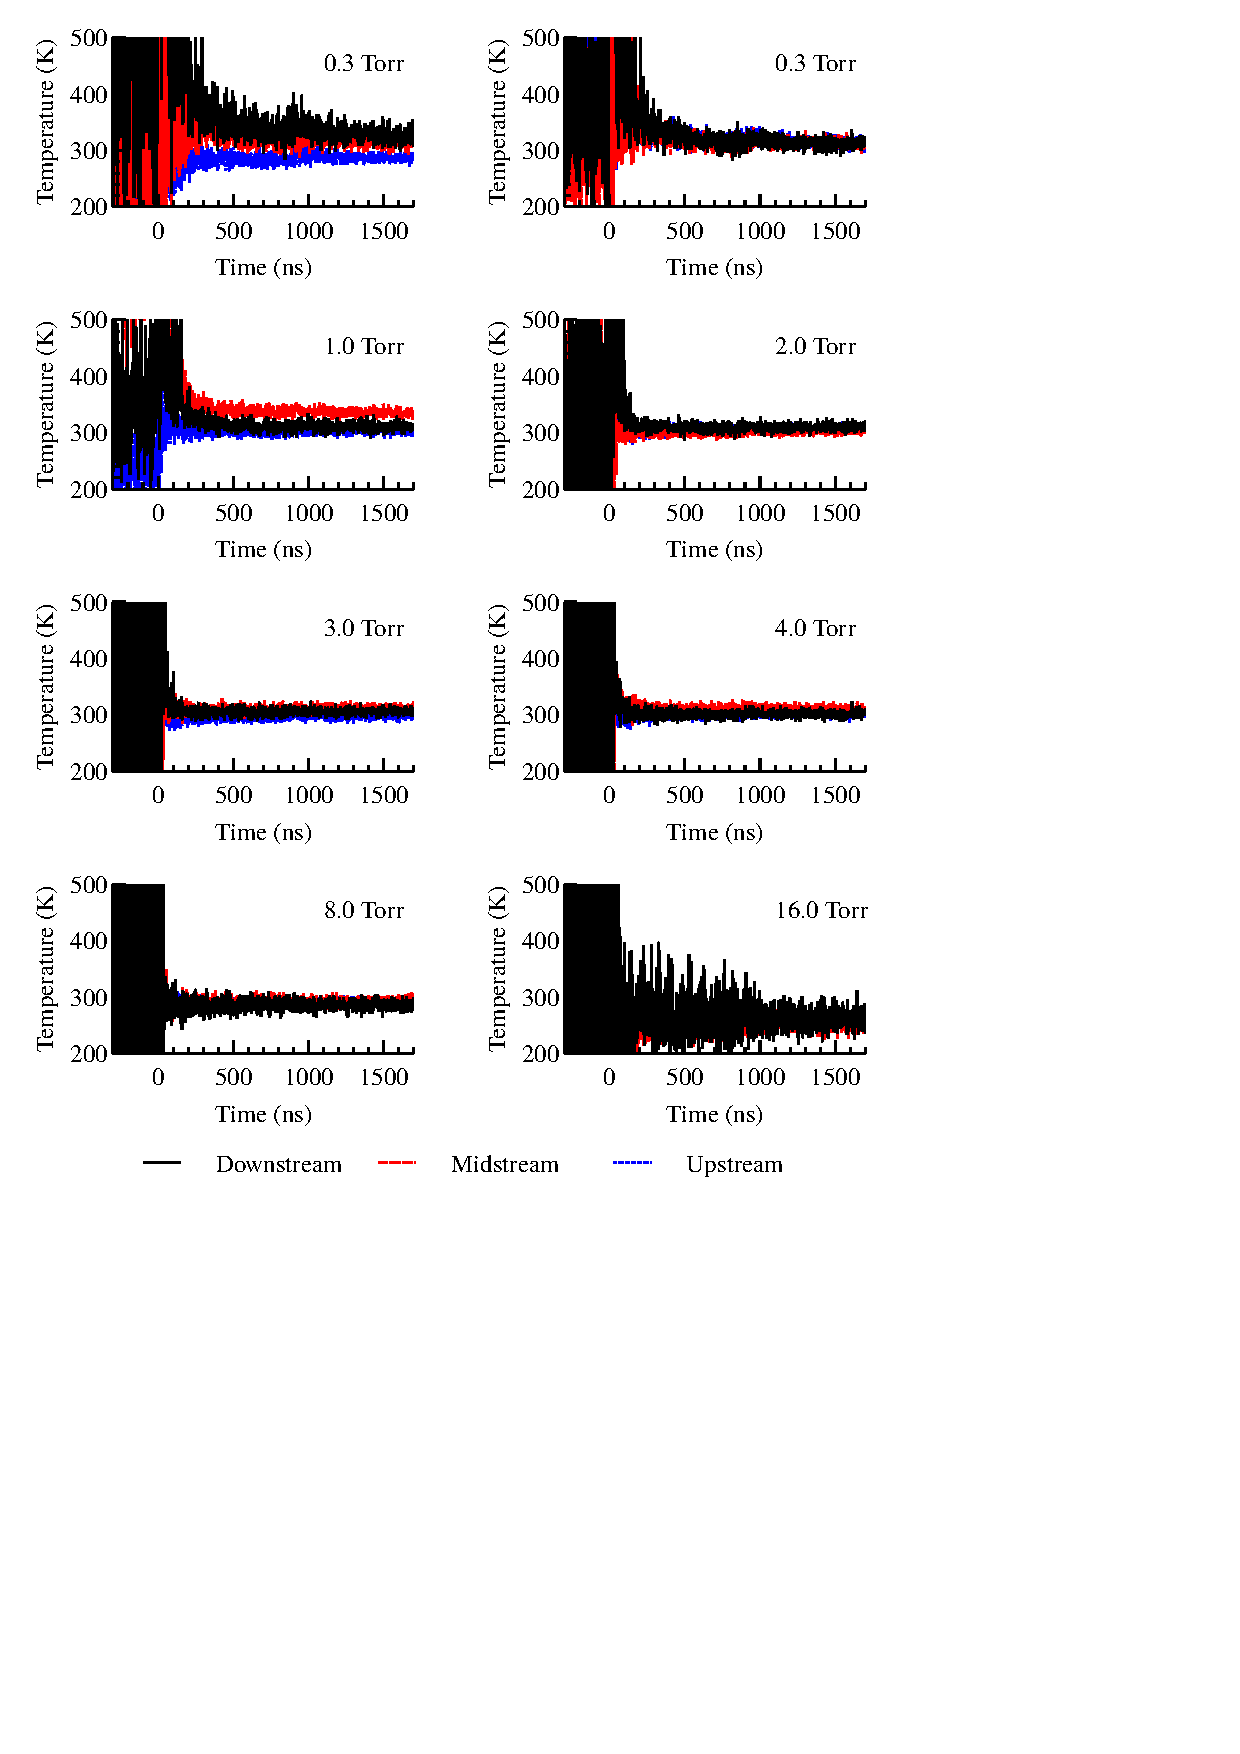
\includegraphics{./chapters/nasa/figures/temperatures.pdf}
  \caption{Rotational temperature trends for three operating conditions:
    $\pm4.3$ (solid black), $\pm6.1$ (dashed red) and $\pm7.3$ kV (dotted blue). The
    first two cases exhibit significant variations near the end of the measurement
    period as a result of low signal-noise ratios. Only $\pm7.3$ kV case shows any
    clear trends over the duration of the measurement.}
  \label{fig:temperatures2}
\end{figure}
Matching temperatures were not found for all time points as, in some cases, the signal was too weak to reliably measure the temperature.

The $\pm7.3$ kV case appears to show a consistent rise in temperature during the
pulse. The signal-noise ratio is too low in the $\pm4.3$ and $\pm6.1$ kV cases
to make a clear determination. Likewise, the $\pm4.3$ and $\pm6.1$ kV case show
little or no decrease for the duration of observation, while the $\pm7.3$ kV
case does appear to show a steady decrease during the observation period. The
peak rotational temperatures ranged from $750$ to $850$ K.

One possibility for downward trend in the $\pm7.3$ kV case is the depletion of
\textsc{c}$^3\Pi_\mathrm{u}$ rotational states with higher $J$ due to the
dissociation of nitrogen molecules. The dissociation energy of molecular
nitrogen is $113\,029$ cm$^{-1}$ and the energy of \textsc{c}$^3\Pi_{\mathrm{u};
\upsilon=0}$ is $88\,977.9$ cm$^{-1}$. Therefore an additional $24\,051.1$
cm$^{-1}$, or approximately $2.98$ eV, is required to dissociate the molecule.
The $\pm7.3$ kV case likely produced a more energetic electron population and,
therefore, would have a greater depletion of the higher rotational states in the
system. This would have prevented those states from transitioning to
\textsc{b}$^3\Pi_\mathrm{g}$ and thus resulted in an artificially low
temperature. Measurements of the effective electron temperature in similar
systems suggests a range of possibilities from $0.6$--$33$ eV
\cite{Aleksandrov2010}, \cite{Takashima2011}, and \cite{Nikandrov2008}.

Relation of the rotational temperatures to kinetic temperatures must be done
carefully on these time scales. In most cases, the rotational temperature
equilibrates with the kinetic temperature much faster than it can change.
Assuming, however, that the kinetic temperature changes on a time scale on the
order of the ionization wave, this is no longer the case. The ionization wave
traverses the length of the discharge in several nanoseconds and may cause an
abrupt increase in kinetic temperature. Equilibration with this change requires
the excited nitrogen molecules undergo several collisions with the neutral gas.
The time between collisions at a temperature of 750 K is approximately 1.5 ns
\cite{Hasegawa1987}. The time resolution of the gas temperature is effectively
several times this number, conservatively 10 ns. Therefore, the initial upward
trend of the $\pm 7.3$ case does not readily translate to an increase in gas
temperature.

It is difficult to quantify the degree of uncertainty associated with these
measurements. The uncertainty is minimal for the largest signals, from
approximately $11$ ns through $30$ ns. Based on the oscillations of the final
temperature measurements in this time period, the random error appears to be on
the order of $\pm50$ K. As the signal strength decreases, this error increases
significantly. In addition, systematic errors were present which may have
affected the matching process. As mentioned, the $(1,1)$ and $(2,2)$ transitions
were not included in the simulations. Additionally, the lack of an intensity
calibration may have influenced the results; the efficiency of the grating may
have changed over the range of wavelengths under investigation. Finally, the
instrument function featured a slightly wider base than the Gaussian used to
represent it.

\section{Conclusions}

The \acs{rpnd} is promising for use in air-breathing hypersonic propulsion as
part of an energy bypass mechanism. However, the successful application of the
\acs{rpnd} required that its electron density and gas heating be measured. Both
of these help to describe its overall efficiency in the ionization of an inlet
airflow.

The electron density and collision frequency were measured as functions of time
using \acs{mmw} interferometry. It was found that the two quantities underwent
significant changes in the first five to ten minutes of operation, after which
the values stayed approximately constant. It is hypothesized that these changes
were a result of evolving chemical composition and temperature in the discharge
chamber, resulting from the use of stagnant air. No evidence was found to
support the claims that the DC sustainer improved the time-average particle
density, however experimental difficulties require that this measurement be
revisited.

Literature suggested that the sustainer and the \acs{rpnd} itself may be
responsible for a significant degree of gas heating. This represents an
important loss mechanism for the applied energy and can impact the downstream
combustion chemistry. Heating in the \acs{rpnd} was analyzed via measurements of
the rotational spectra in the system. A program was written to automatically
generate synthetic spectra for a variety of conditions and then to pick the one
most appropriate for a measured spectrum. It was found that the temperature of
the \acs{rpnd} was reliably between 750-850 K. A decline in temperature was
observed for the case with the highest bias. It is believed that this was caused
by a depletion of the higher rotational states due to dissociation, resulting in
an artificially lower temperature.
